\hypertarget{_input_thread_8cpp}{\section{/home/travis/build/bender-\/wardrobe/\-Recast/src/threads/\-Input\-Thread.cpp File Reference}
\label{_input_thread_8cpp}\index{/home/travis/build/bender-\/wardrobe/\-Recast/src/threads/\-Input\-Thread.\-cpp@{/home/travis/build/bender-\/wardrobe/\-Recast/src/threads/\-Input\-Thread.\-cpp}}
}


Input thread for execution of terminal command.  


{\ttfamily \#include $<$string$>$}\\*
{\ttfamily \#include $<$iostream$>$}\\*
{\ttfamily \#include $<$boost/log/trivial.\-hpp$>$}\\*
{\ttfamily \#include \char`\"{}threads/\-Input\-Thread.\-hpp\char`\"{}}\\*
{\ttfamily \#include \char`\"{}Server.\-hpp\char`\"{}}\\*
Include dependency graph for Input\-Thread.\-cpp\-:
\nopagebreak
\begin{figure}[H]
\begin{center}
\leavevmode
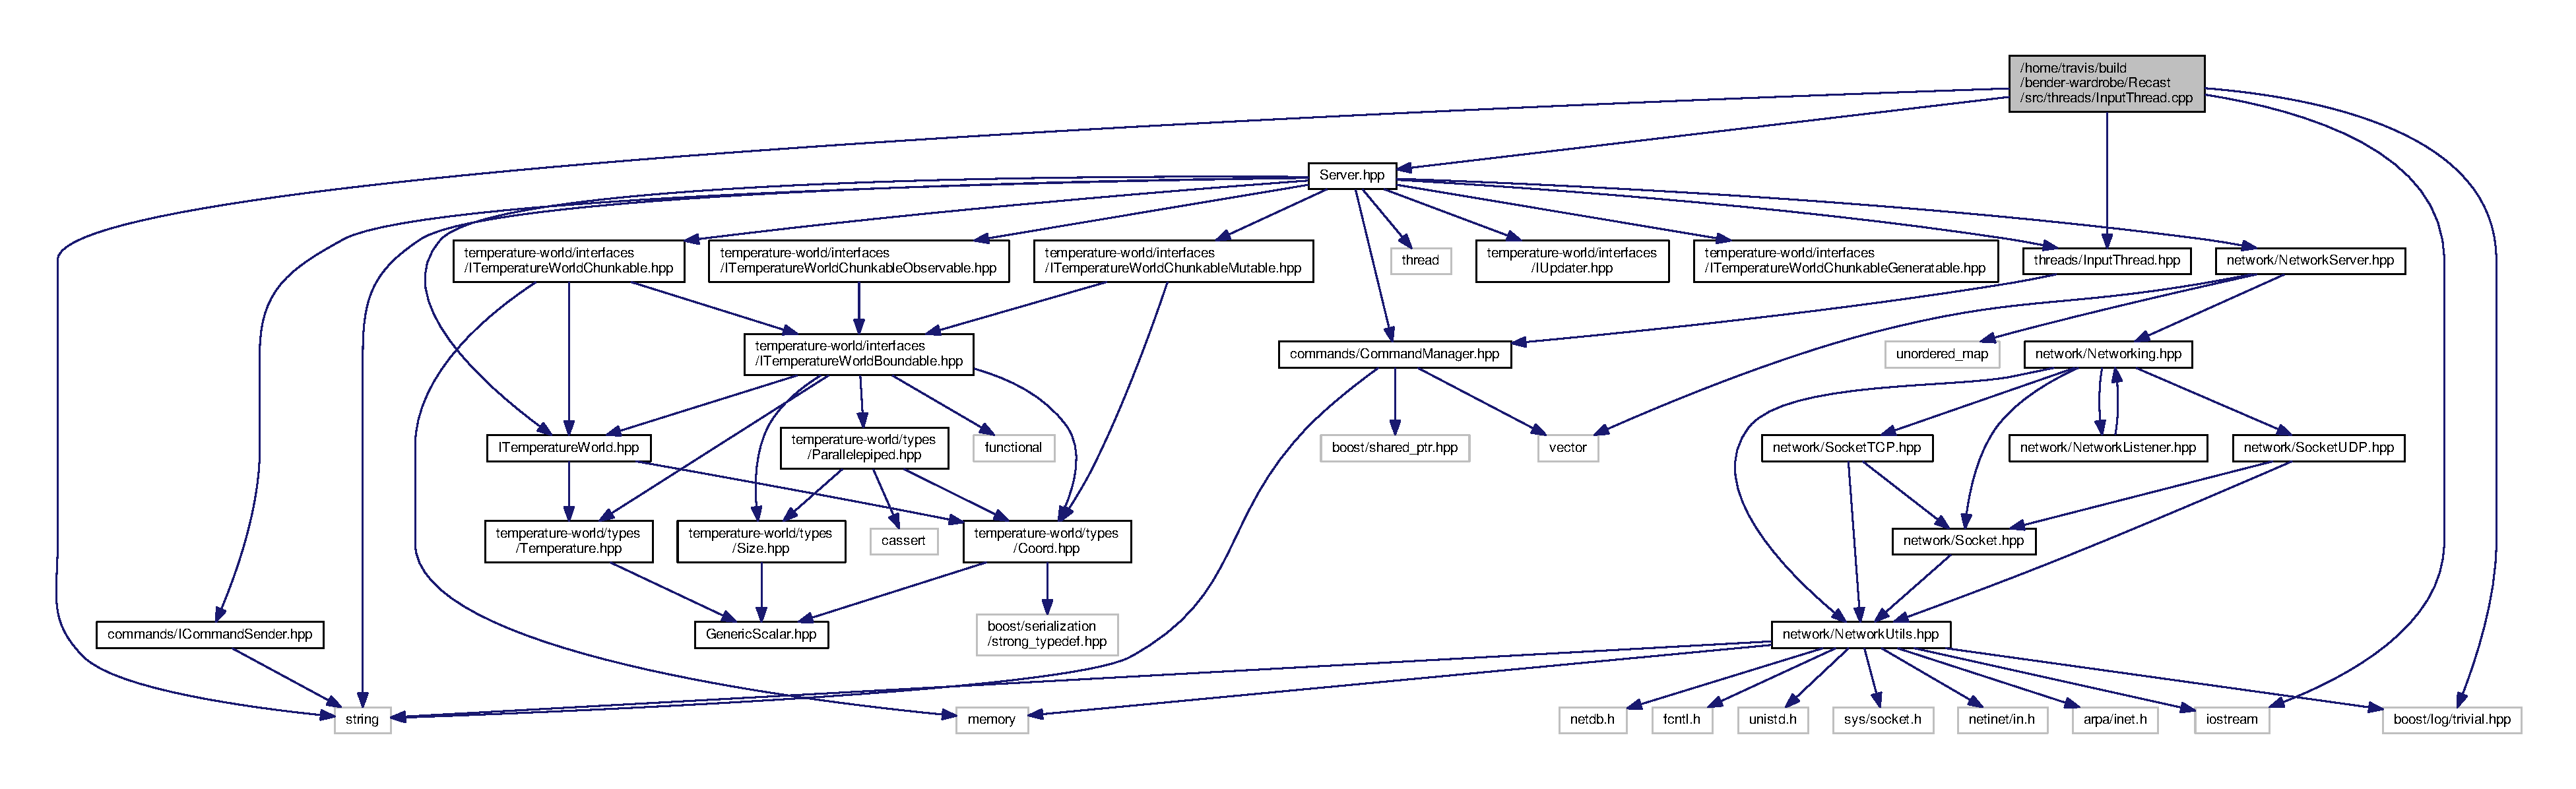
\includegraphics[width=350pt]{_input_thread_8cpp__incl}
\end{center}
\end{figure}


\subsection{Detailed Description}
Input thread for execution of terminal command. \begin{DoxyAuthor}{Author}
Lion\-Z\-X\-Y  Recast-\/server 
\end{DoxyAuthor}
\begin{DoxyDate}{Date}
12.\-06.\-17  \href{mailto:nikita@kulikof.ru}{\tt nikita@kulikof.\-ru}
\end{DoxyDate}
Execute background command 